\documentclass[10pt]{beamer}

\usetheme[progressbar=frametitle]{metropolis}
\usepackage{appendixnumberbeamer}

\usepackage{booktabs}
\usepackage[scale=2]{ccicons}

\usepackage{pgfplots}
\usepgfplotslibrary{dateplot}

\usepackage{amssymb}
\usepackage{amsmath}
\usepackage{amsthm}
\usepackage{mathabx}

\usepackage{float}
\setlength{\leftmargini}{0pt}

\usepackage{bbm}
\usepackage{pgf, tikz}
\usetikzlibrary{positioning}
\usepackage{tcolorbox}

\newtheorem*{assumption}{Assumption}

\usepackage{xspace}
\newcommand{\themename}{\textbf{\textsc{metropolis}}\xspace}
\DeclareMathOperator*{\E}{\mathbb{E}}
\DeclareMathOperator*{\R}{\mathbb{R}}
\DeclareMathOperator*{\Var}{\mathbb{V}ar}
\DeclareMathOperator{\fa}{\hspace{.1cm} \forall \hspace{.1cm}}
\newcommand{\wh}{\widehat}
\newcommand{\wtl}{\widetilde}
\def\argmin{\mathop{\textrm{argmin}}}
\def\1{\mathop{\mathbbm 1}\nolimits}
\newcommand{\Ex}{{\mathbb E}}
\newcommand{\PP}{\mathbb{P}}

\setbeamertemplate{theorems}[numbered] 
\newtheorem*{remark}{Remark} 
\newtheorem*{defin}{Definition}
\newtheorem*{thm}{Theorem}
\newtheorem*{ex}{Example}

\makeatother

\title{Is More Information Better? The Effects of "Report Cards" on Health Care Providers}
\subtitle{David Dranove et al.}

\date{October 24, 2022}
\author{Jung Jae Kim}

\begin{document}
\lecture{Test lecture one}{lone}

\maketitle
%Start of the document

\begin{frame}{Motivation}

\begin{itemize}
\item \textbf{"Report cards"}: provide information about the performance. 
\item Debate on the merits of report cards
\item Supporters: Patients can identify the best physicians and hospitals. 
\item Skeptics: Providers select healthier patients to improve their ranking.
    \begin{itemize}
        \item [(1)] Asymmetric information
        \item [(2)] The significant difference in outcomes
        \item [(3)] The utility loss from a few bad outcomes
    \end{itemize}
\end{itemize}

\begin{itemize}
    \item[] \textbf{Research objective}: Assessing the competing claims about report card.
    \begin{itemize}
        \item[1.] The matching of patients to providers.
        \item[2.] The incidence and quantity of CABG surgeries.
        \item[3.] The incidence and quantity of complementary and substitute treatments.
    \end{itemize}
\end{itemize}

\end{frame}

\begin{frame}{Preview of the Main Results}

\begin{itemize}
\item Improved matching of patients with hospitals
\item Increased the quantity of CABG surgery.
\item Changed its incidence from sicker patients toward healthier patients.
\item Overall, this led to higher costs and a deterioration of outcomes.
\end{itemize}

\end{frame}

\begin{frame}{History of health care report cards}

\begin{itemize}
\item Two "treatment" states: \\Only NY and PA reported outcomes for patients receiving CABG
\item Beginning in 1990, NY released raw and risk-adjusted CABG mortality.
\item Beginning in November 1992, PA published data on risk-adjusted CABG mortality.
\item Report cards could have begun to affect decision making in NY in 1991 and PA in 1993.
\end{itemize}

\end{frame}

\begin{frame}{Empirical Models}
\begin{itemize}
\item[A.] \textit{Hospital-Level Analysis}
\begin{equation}
\ln \left(h_{l s t}\right)=\mathbf{A}_s+\mathbf{B}_t+g \cdot \mathbf{Z}_{l s t}+p \cdot L_{s t}+q \cdot N_{s t}+e_{l s t},
\end{equation}
             \begin{align*}
                h_{lst}&: \; \text{mean of the illness severity before treatment of hospital $l$}\\
                \mathbf{A}_s&: \; \text{State fixed effects}\\
                \mathbf{B}_t&: \; \text{Time fixed effects}\\
                \mathbf{Z}_{lst}&: \; \text{Hospital Characteristics}\\
                L_{st}&: \; \text{1 if the hospital is in treatment groups}\\
                N_{st}&: \; \text{The number of hospitals, and its square and cube}
            \end{align*}
\item If $p<0$, then report cards caused a shift in incidence from sicker to healthier patients.
\item Reestimate equation (1) for AMI patients who are not subject to selection.
\item Reestimate equation (1) using the within-hospital coefficient of variations; an estimated $p<0$ is consistent with improved patient sorting.
\end{itemize}

\end{frame}

\begin{frame}{Empirical Models}
\begin{itemize}
\item[B.] \textit{Patient-Level Analysis}
\begin{equation}
C_{k s t}=\mathbf{A}_s+\mathbf{B}_t+g \cdot \mathbf{Z}_{k s t}+p \cdot L_{s t}+e_{k s t}
\end{equation}
             \begin{align*}
                C_{kst}&: \; \text{1 if patient $k$ received CABG within one year of admission for AMI}\\
                \mathbf{A}_s&: \; \text{State fixed effects}\\
                \mathbf{B}_t&: \; \text{Time fixed effects}\\
                \mathbf{Z}_{kst}&: \; \text{Patient Characteristics}\\
                L_{st}&: \; \text{1 if patient $k$'s residence is in treatment groups}
            \end{align*}
\item If $p>0$, then report cards increased the probability that an AMI patient receives CABG.
\item Reestimate (2) for alternative treatments PTCA and cath.
\end{itemize}

\end{frame}

\begin{frame}{Empirical Models}
\begin{itemize}
\item[B.] \textit{Patient-Level Analysis}
\item Let $O_{kst}$ be one if patient $k$ experienced an adverse health outcome. Reestimate (2) with $O_{kst}$.
\item  Let $y_{kst}$ be his total hospital expenditure after admission with AMI. Reestimate (2) with $ln(y_{kst})$.
\item If report cards uniformly decrease adverse outcomes and decrease costs, then we conclude their effect on social welfare is positive.
\end{itemize}

\end{frame}

\begin{frame}{Data}
\begin{itemize}
\item Medicare claims data from 1987 to 1994.
\item As a measure of the patient's illness severity before treatment, total inpatient hospital expenditures for the year prior to admission are used.
\item As a measure of the intensity of treatment, total inpatient hospital expenditures in the year after admission are used.
\item Data on U.S. hospital characteristics are from American Hospital Association. 
\end{itemize}

\end{frame}

\begin{frame}\frametitle{Hospital-Level Analysis}
\setlength{\leftmargini}{12pt}
\vspace{-7.5mm}
 \begin{figure}[h!]
        \centering
        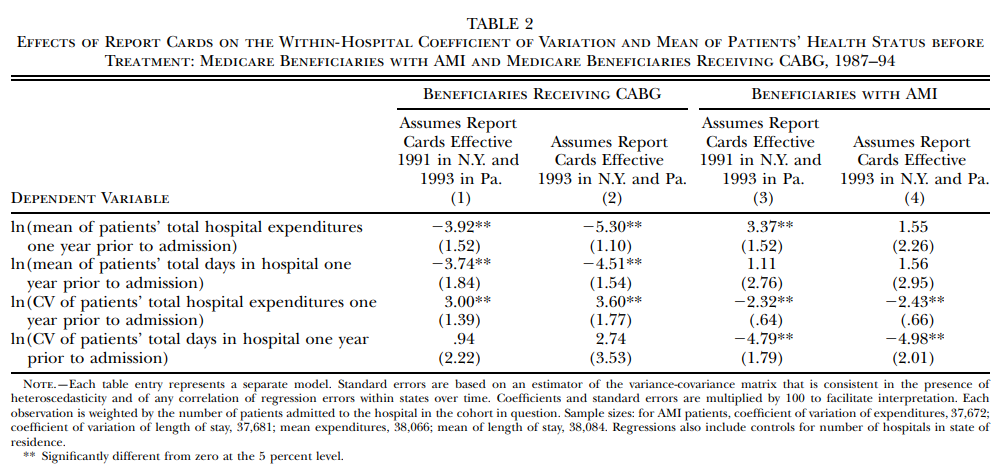
\includegraphics[width=112mm]{table1.png}
        \label{fig:method}
        \end{figure}
        \vspace{-9.5mm}

\end{frame}

\begin{frame}\frametitle{Patient-Level Analysis}
 \begin{figure}[h!]
        \centering
        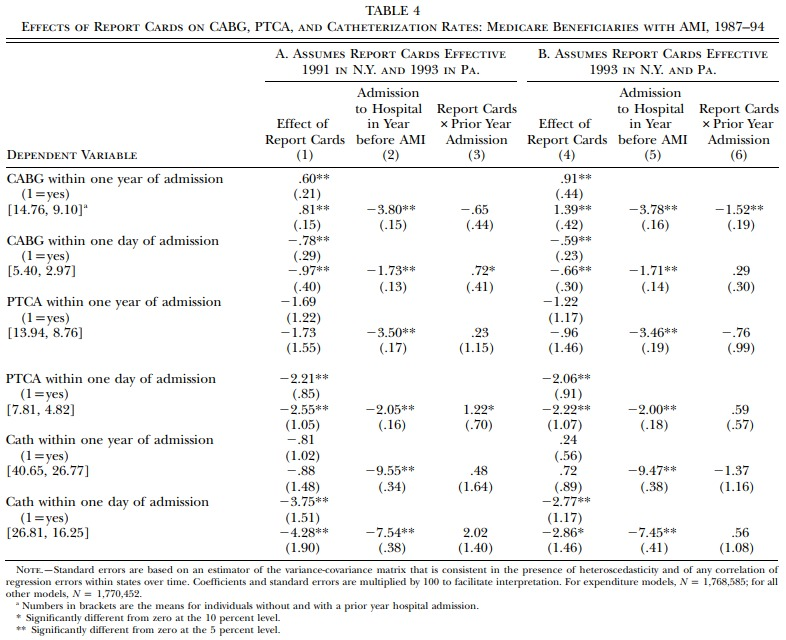
\includegraphics[width=100mm]{table2.jpg}
        \label{fig:method}
        \end{figure}
\end{frame}

\begin{frame}\frametitle{Patient-Level Analysis}
 \begin{figure}[h!]
        \centering
        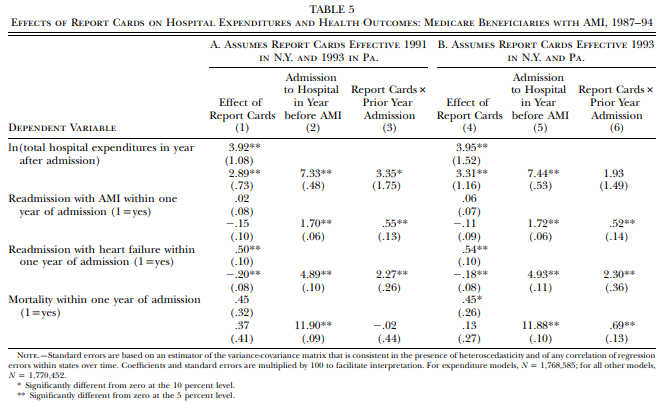
\includegraphics[width=110mm]{table3.png}
        \label{fig:method}
        \end{figure}
\end{frame}

\begin{frame}\frametitle{Conclusion}
\setlength{\leftmargini}{12pt}

\begin{itemize}
    \item [1.] CABG surgery report cards led to substantial selection by providers.
    \item [2.] Report cards led to increased sorting of patients to providers.
    \item [3.] Report cards reduced the measure of welfare, higher levels of Medicare hospital expenditures and greater rates of adverse health outcomes.
\end{itemize}
    \begin{itemize}
        \item[] \textbf{Cautions}
    \begin{itemize}
        \item [(1)] Measure only short-run responses.
        \item [(2)] The results do not imply that report cards are harmful in general.
        \item [(3)] Report cards and the incentives they create are not unique to health care. 
    \end{itemize}
    \end{itemize}

\end{frame}




\end{document}